\chapter{Prezentacja aplikacji}
Interfejs użytkownika składa się z elementów, które pozwalają w płynny sposób poruszać się po aplikacji oraz dostosowywać ją do własnych potrzeb. Celem tego rozdziału jest zaprezentowanie funkcjonalności w warstwie prezentacji.
\section{Środowisko deweloperskie}
Aplikacja webowa uruchamiana jest w środowisku deweloperskim. Urządzenie, na którym uruchomiona jest aplikacja działa jak serwer i klient jednocześnie. Odwołanie do lokalnego hosta (\textit{localhost}) jest wymagane by uruchomić aplikację, która znajduje się domyślnie pod adresem \texttt{localhost:5173/}, gdzie liczba po dwukropku oznacza port z którego korzysta aplikacja. W dalszej części rozdziału adres zostanie zastąpiony słowem ,,\texttt{HOST}''.

\section{Formularze autoryzacji}
Po pierwszym załadowaniu aplikacji www użytkownik zostanie przekierowany przez system do formularza logowania znajdującego się pod adresem \texttt{HOST/auth/login}. Zawiera on dwa pola wymagane, w których użytkownik powinien podać nazwę użytkownika oraz hasło, i pole wyboru umożliwiające zapisanie danych (rys. \ref{fig:login}). Użytkownik który nie posiada konta ma możliwość utworzenia go poprzez kliknięcie w odnośnik \textit{Zarejestruj się!}, który przenosi do formularza rejestracji.
\section{Ustawienia użytkownika}
Aplikacja webowa oferuje możliwość personalizacji strony poprzez zakładkę ustawień (rys. \ref{fig:ustawienia}) znajdującą się po prawej stronie na pasku nawigacyjnym (ang. \textit{navbar})(rys. \ref{fig:navbar}). Aplikacja pozwala na ustawienie ciemnego oraz jasnego wygląd interfejsu użytkownika (rys. \ref{fig:motywy}) oraz zmianę języka na polski lub angielski (rys. \ref{fig:login})
\begin{figure}[H]
\begin{minipage}{0.5\textwidth}
	\centering
	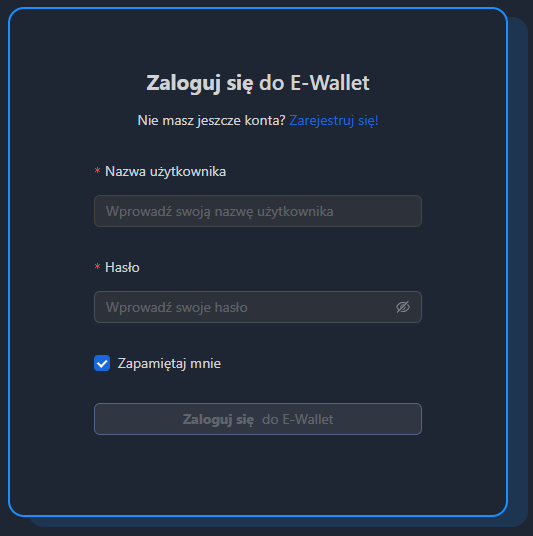
\includegraphics[width=\linewidth]{images/Login}
\end{minipage}
\hfill
\begin{minipage}{0.5\textwidth}
	\centering
	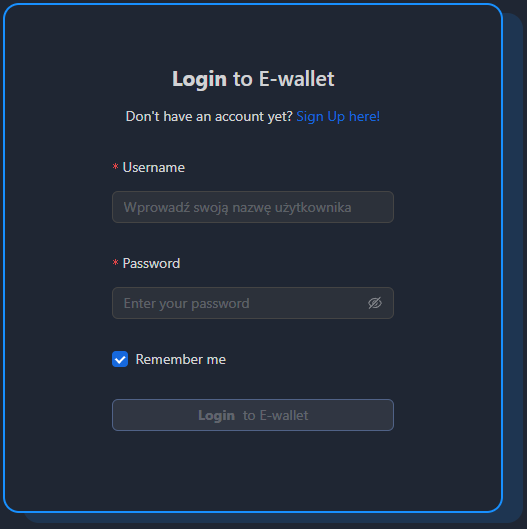
\includegraphics[width=\linewidth]{images/LoginAng}
\end{minipage}
	\caption{Formularz logowania po polsku i angielsku}
	\label{fig:login}
\end{figure}
\begin{figure}[H]
	\centering
	
\includegraphics[width=0.6\linewidth]{images/Navbar}
	\caption{Pasek nawigacyjny}
	\label{fig:navbar}
\end{figure}

\begin{figure}[H]
    \begin{minipage}{0.5\textwidth}
	\centering
	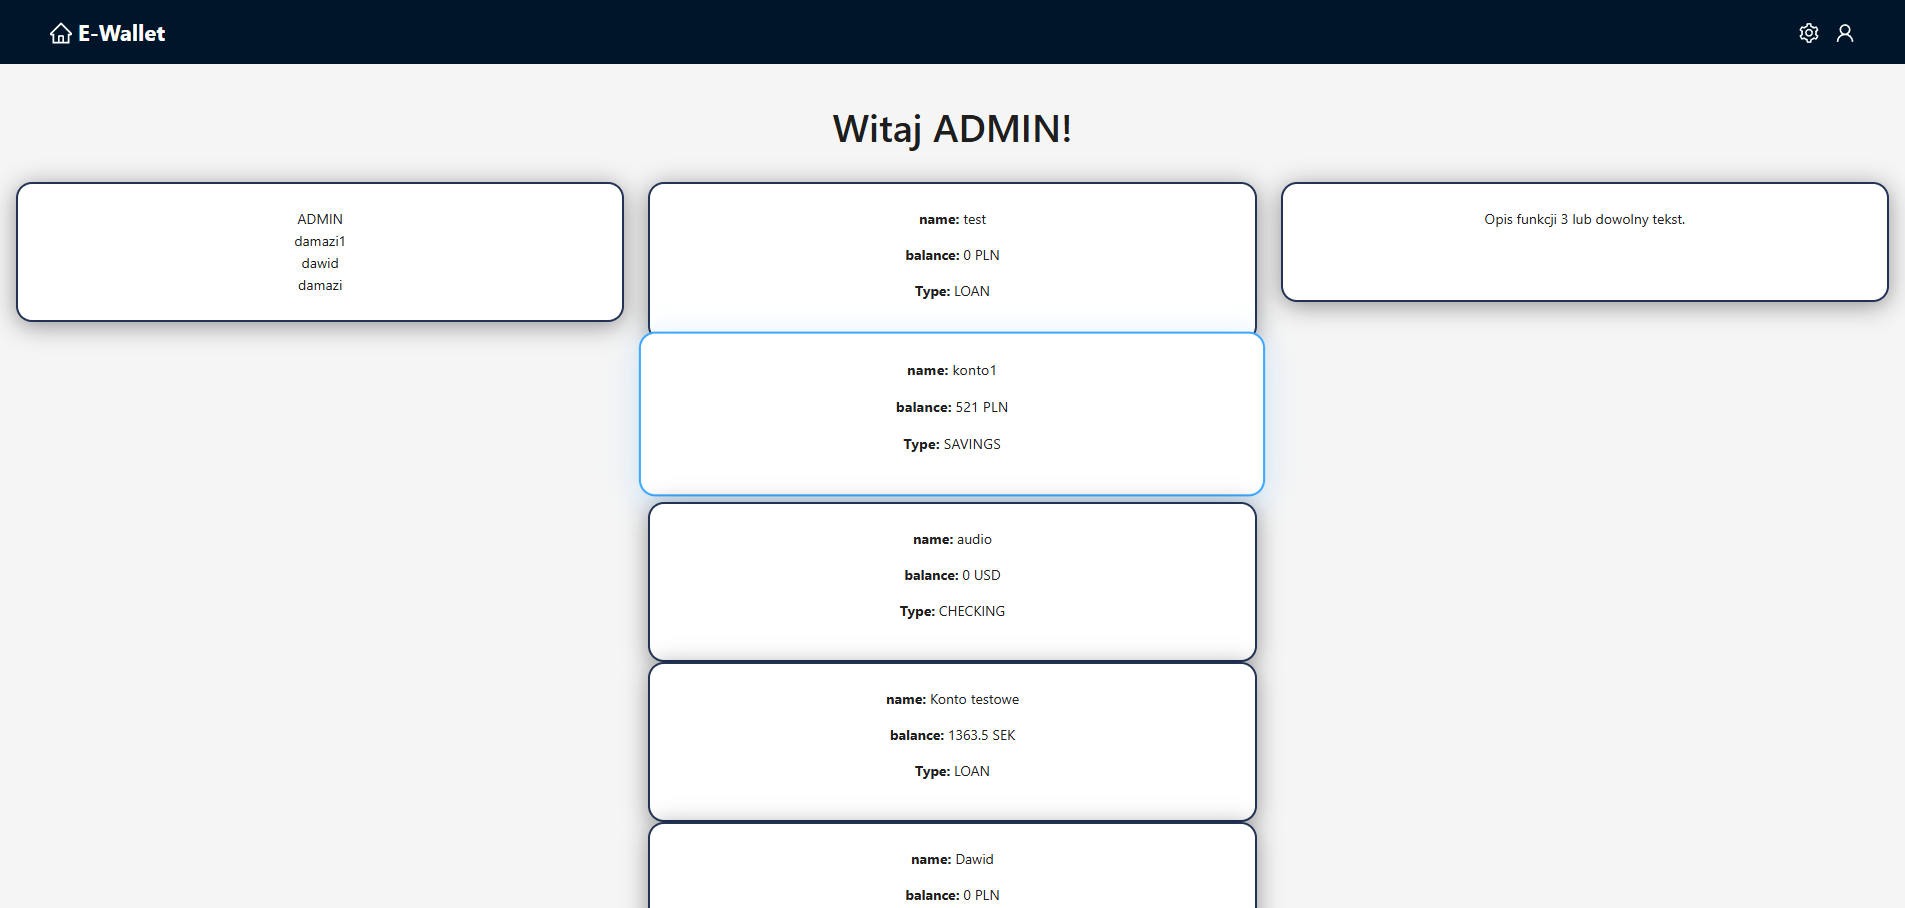
\includegraphics[width=\linewidth]{images/MotywJasny}
\end{minipage}
\hfill
\begin{minipage}{0.5\textwidth}
	\centering
	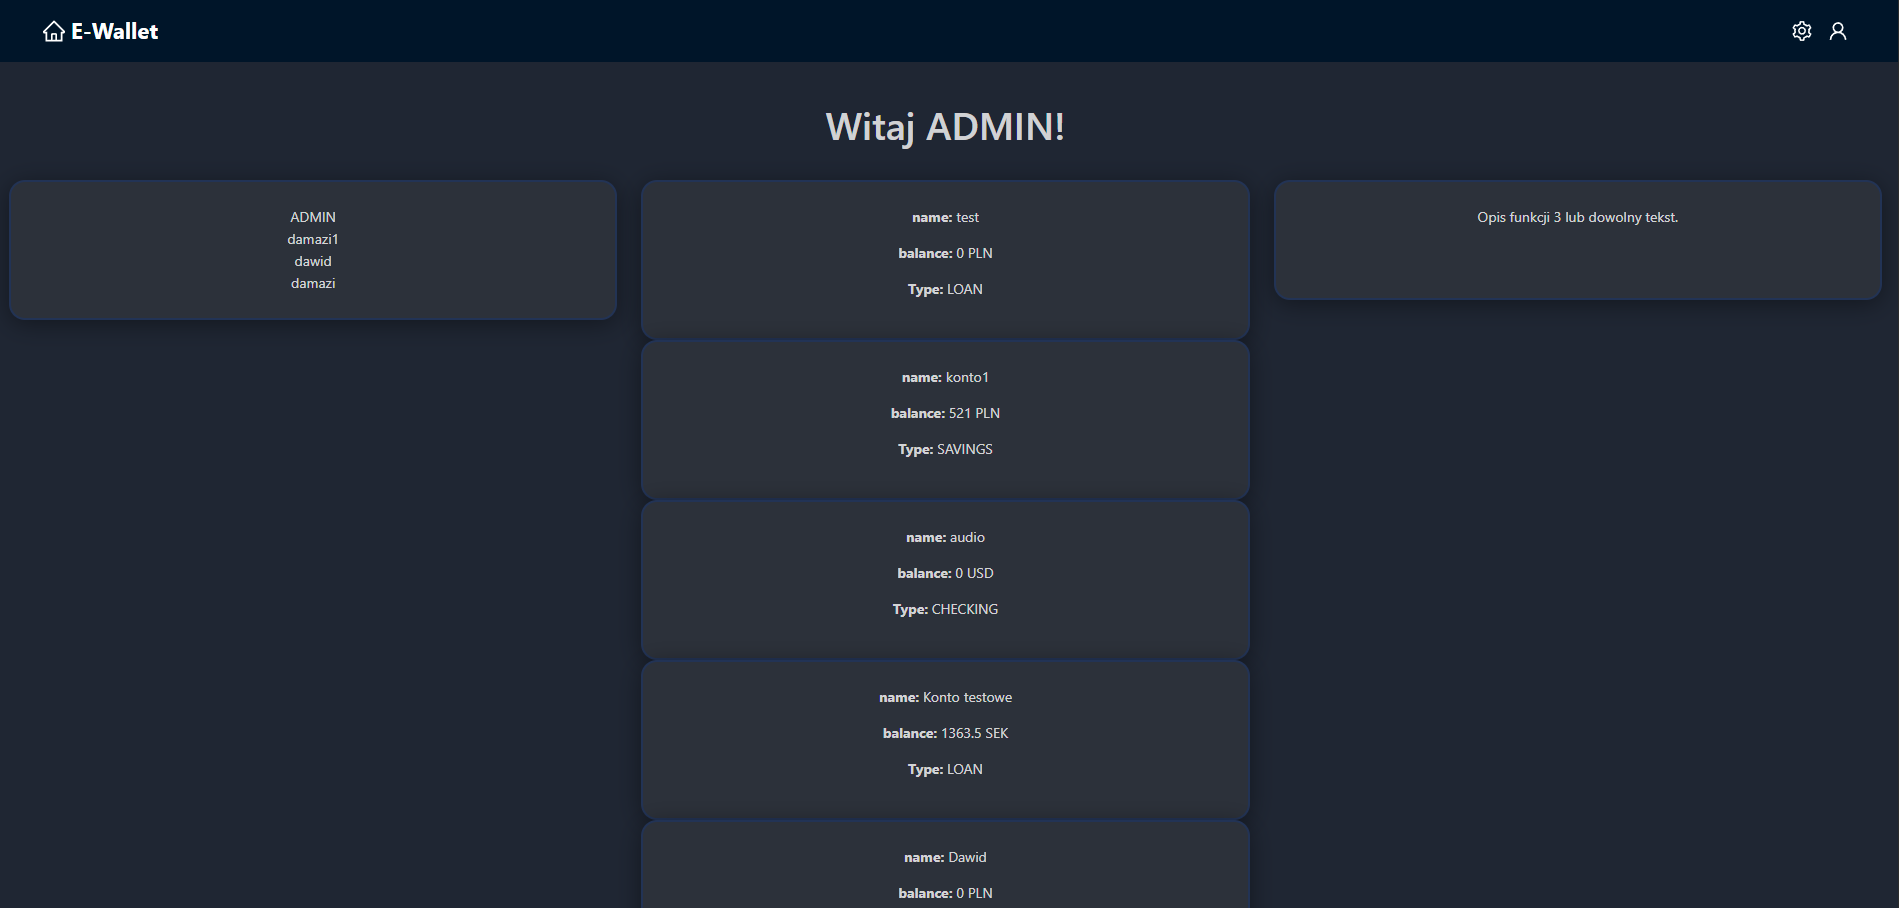
\includegraphics[width=\linewidth]{images/MotywCiemny}
\end{minipage}
	\caption{Motywy strony}
	\label{fig:motywy}
\end{figure}

\begin{figure}[H]
	\centering
	
\includegraphics[width=0.7\linewidth]{images/Ustawienia}
	\caption{Ustawienia użytkownika}
	\label{fig:ustawienia}
\end{figure}
\section{Funkcjonalność aplikacji udostępniona użytkownikowi zalogowanemu}
Pomyślna próba logowania spowoduje przekierowanie do strony głównej. System powita użytkownika oraz wypiszę wszystkie portfele aktualnego klienta w postaci kafelków, po których kliknięciu nastąpi przekierowanie do strony danego portfela. Pojawi się również możliwość sprawdzenia szczegółów konta oraz wylogowania po prawej stronie paska nawigacyjnego. 
\subsection*{Szczegóły konta}
Użytkownik może wyświetlić informację o swoim koncie oraz dodać nowe portfele. Dodatkowo jeżeli użytkownik posiada rolę administratora może edytować konta innych użytkowników oraz nadawać uprawnienia.
\\Adres pod którym znajduje się podstrona to \texttt{HOST/details/\{Nazwa\_Użytkownika\}}
\subsection*{Portfel użytkownika}
Klient ma możliwość zarządzania oraz wyświetlania szczegółu na temat portfela. Dane transakcji są przedstawione na wykresach, które umożliwiają wyświetlanie wszystkich transakcji lub podsumowania za każdy dzień (rys. \ref{fig:wykresy}). Użytkownik ma możliwość odczytania informacji o nazwie swojego portfela, ilości dostępnych środków i typie konta. Dostępne są również operację takie jak wpłata, wypłata i przelew (rys. \ref{fig:daneportfela}). Wybranie jednej z operacji otworzy okno modalne wymagające uzupełnienia danych. Ostatnim elementem jest historia wszystkich transakcji, która zawiera kwotę, datę, numer portfela, z którego została wykonana transakcja i numer odbiorcy transakcji oraz status (rys. \ref{fig:transakcjehistoria}). 
\begin{figure}[H]
	\begin{minipage}{0.5\textwidth}
	\centering
	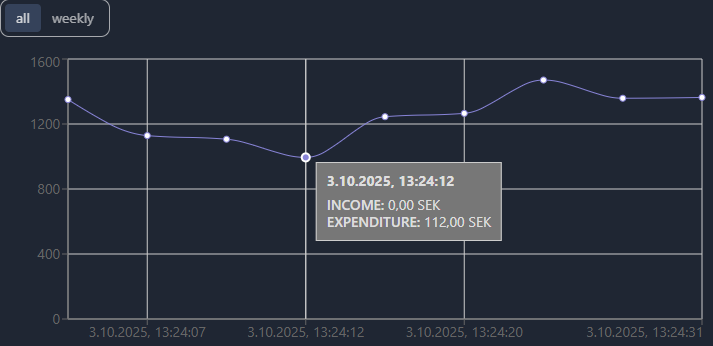
\includegraphics[width=\linewidth]{images/TransakcjeAll}
\end{minipage}
\hfill
\begin{minipage}{0.5\textwidth}
	\centering
	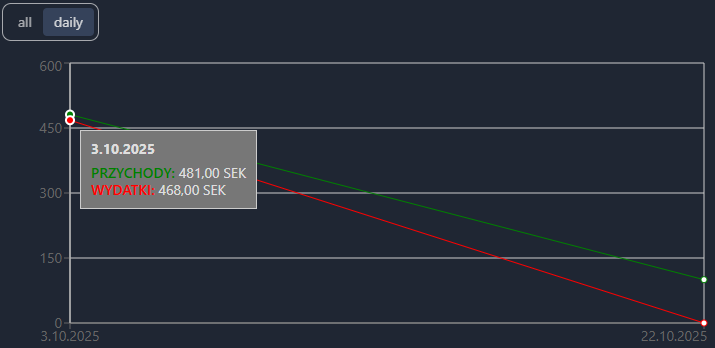
\includegraphics[width=\linewidth]{images/TransakcjeDaily}
\end{minipage}
	\caption{Wykresy wpływów i wypłat z portfela}
	\label{fig:wykresy}
\end{figure}

\begin{figure}[H]
		\begin{minipage}{0.5\textwidth}
	\centering
	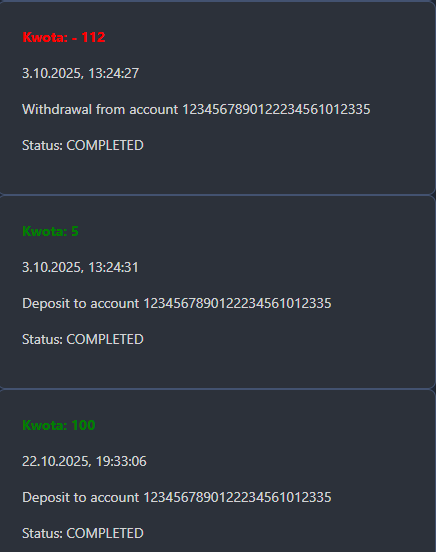
\includegraphics[width=0.7\linewidth]{images/TransakcjeHistoria}
	\caption{Historia transakcji}
	\label{fig:transakcjehistoria}
\end{minipage}
\hfill
		\begin{minipage}{0.5\textwidth}
	\centering
	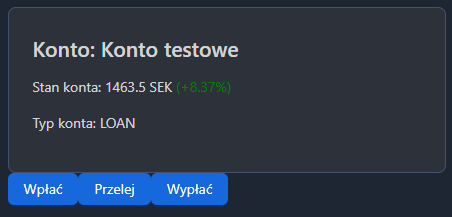
\includegraphics[width=\linewidth]{images/DanePortfela}
	\caption{Dane portfela}
	\label{fig:daneportfela}
\end{minipage}
\end{figure}
